% -*- TeX -*- -*- UK -*- -*- Soft -*-


\part{Bayesian Algorithms}

\chapter{Bayesian Overview}
\label{chap:BayesianOverview}

\section{Frequentist vs. Bayesian Approach}

\newthought{In the frequentist approach} probabilities are defined by the frequency of countable events in the limiting case of repeated measurements (sampling distribution) of very large samples.
In the frequentist view it is meaningless to talk of the probability \textit{of the true value} of something: such a true value is a single fixed value  and cannot have a probability/frequency distribution.  Deviations from the true value are attributable to measurement inaccuracy or noise.
This means that parameters and models cannot have probability distributions, only measurements can. 
For the frequentist (measurement) uncertainty can only be observed by resampling the process, because the true value is always fixed. This resampling is often not possible or never done.\cite{McElreath2015,vanderPlasFreqBayes2014}

\newthought{For Bayesians}, probabilities are fundamentally related to our own knowledge about an event, i.e., counting the numbers of ways things can happen, \textit{but according to additional assumptions beyond the count frequency}. This probability may/will include measurements  of the frequencies of countable events, but is not limited to frequency measurements as the only and fundamental source of information. Bayesian probability codifies our knowledge of the value based on measured observations and/or  prior information\marginnote{The prior is the probability of an event before witnessing any data.}.  There is no single true value (as frequentists  insist), but rather the plausibility of different possibilities. In the Bayesian view, we can talk about the probability that the true value of something falls in a given range. Probability therefore now  has a wider meaning: as the representation of  plausibility, or the degree of certainty about events.  This concept of plausibility applies not only to the measured count frequency, but also applies to models or parameters.
 \cite{McElreath2015,vanderPlasFreqBayes2014}

\newthought{Probability is not unitary.} It will make some readers uncomfortable to suggest that
there is more than one way to define ''probability.'' Aren’t mathematical concepts uniquely correct?
They are not. Once you adopt some set of premises, or axioms, everything does follow logically in
mathematical systems. But the axioms are open to debate and interpretation. So not only is there
''Bayesian'' and ''frequentist'' probability, but there are different versions of Bayesian probability even, relying upon different arguments to justify the approach.\cite{McElreath2015}

\section{Counting Balls the Frequentist Way}
\label{sec:CountingBalls}
\subsection{The Frequentist Way}
\label{sec:TheFrequentistWay}

McElreath \cite{McElreath2015} considers the problem of drawing coloured balls from a bag.  The bag is known to contain four balls, either white (W) or blue (B).  Three balls are drawn from the bag, the colour noted and the ball returned to the bag: on each draw there will be the same four balls in the bag.

Three balls are drawn as follows: BWB (blue, white, blue). What is the contents of the bag, how many white balls and how many blue balls?  There are five different conjectures and for each of these conjectures the number of ways to produce the draw is shown in the figure.
\begin{marginfigure}
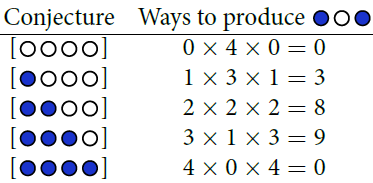
\includegraphics{p05c01-01}
\end{marginfigure}
The ways to produce the draw is found by multiplying for each conjecture the number of possible ways that each of the drawn balls could appear.  The draw produced blue and while balls, hence the first and the last conjecture are unable to produce the observed draw (0 ways). For each of the remaining conjectures the number of production ways are non-zero, reaching a maximum of nine, for the BBBW conjecture --- clearly this is the most plausible (but certainly not the only) bag contents.  At a much lower likelihood the BWWW bag contents could also produce the observed draw.
By normalising ($n$/(0+3+8+9+0)) for the number of ways, the likelihood for the bag contents is
WWWW=0\%, 
BWWW=15\%,
BBWW=40\%,
BBBW=45\%, and
BBBB=0\%.  These values represent the certainty we have for each of the conjectures.

\subsection{Using Prior Information}
\label{sec:UsingPriorInformation}

Using the results from the first three draws above, and we draw a fourth ball, what can we learn about the bags?  Suppose the fourth ball is blue (B).  Extend the previous calculation, and note how many ways a blue ball can be drawn.
\begin{marginfigure}
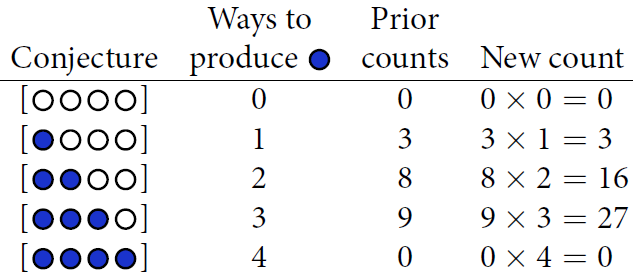
\includegraphics{p05c01-02}
\end{marginfigure}
Then multiply each of these new counts by the prior numbers of ways for each conjecture.  The diagram shows the bag contents likelihood if  drawing the following four balls:  BWBB.
In this example the prior information is the first three balls drawn, the prior data and the new draw are of the same type (balls drawn).  Prior information may also arise from other sources, not just previous draws.

McElreath \cite{McElreath2015} continues his example by informing that 
someone from the marble factory tells you that blue marbles are rare. So for every bag containing BBBW, they made two bags containing BBWW and three bags containing BWWW. They also ensured that every bag contained at least one blue and one white marble.
This prior information is multiplied with the counts after the four balls drawn thus far.
\begin{marginfigure}
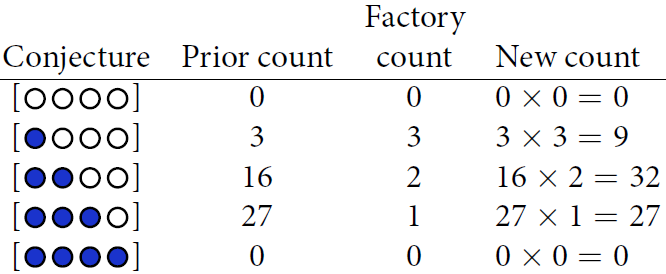
\includegraphics{p05c01-03}
\end{marginfigure}
By normalising ($n$/(0+9+32+27+0)) for the number of ways, the likelihood for the bag contents, based on four draws and the factory prior information, is
WWWW=0\%, 
BWWW=13.2\%,
BBWW=47.1\%,
BBBW=39.7\%, and
BBBB=0\%.  These values represent the certainty we have for each of the conjectures.

How is prior information obtained?  Prior information can be based on previous data (previous draws in this case), but more often on 'other' sources of information, such as a model of the process or the problem context. In the absence of prior information, unity values (a.k.a. 'flat priors') can be assumed.  McElreath  calls this the \textit{Principle of Indifference} or \textit{Ignorance Priors}: When there is no reason to say that one conjecture is more plausible than another, weigh all of the conjectures equally. ``The principle of indifference results in inferences very comparable to mainstream non-Bayesian approaches [i.e., frequentist], most of which contain implicit equal weighting of possibilities. For example a typical non-Bayesian confidence interval weighs equally all of the possible values a parameter could take, regardless of how implausible some of them are.''\cite{McElreath2015}  Although McElreath ``does not endorse ignorance priors'' many problems use such ignorance or flat priors as starting values, and update these as the problem is developed or better understood.


%%%%%%%%%%%%%%%%%%%%%%%%%%%%%%%%%%%%%%%%%%%%%%%%%%%%%%%%%%%%%%%%%%%%%
%%%%%%%%%%%%%%%%%%%%%%%%%%%%%%%%%%%%%%%%%%%%%%%%%%%%%%%%%%%%%%%%%%%%%
%%%%%%%%%%%%%%%%%%%%%%%%%%%%%%%%%%%%%%%%%%%%%%%%%%%%%%%%%%%%%%%%%%%%%
\clearpage
\TBC{To be completed from here onwards}

\lstinline{https://frnsys.com/ai_notes/foundations/bayesian_statistics.html}

\lstinline{https://frnsys.com/ai_notes/machine_learning/bayesian_learning.html}


\section{Defining the Problem}

\newthought{Allen Downey's 2019 SciPy tutorial} lists this approach to defining the problem in Bayes terms:

\begin{enumerate}
\item That are the parameters?  What is my system? What am I trying to estimate?
What is the quantity that I want to know?

\item What are the hypotheses?
What are the possible values for those parameters?


\item What is the prior?
What do I know about the domain before I see the outcome of the experiment?


\item What is the likelihood function?
If someone tells me the hypothetical parameters, can I compute the probability of the data?
What it the probability of my data if I knew what the parameters were?

\end{enumerate} 